\documentclass[11pt]{article}

\usepackage{amsmath}
\usepackage{amssymb}
\usepackage{cite}
\usepackage{hyperref}
\usepackage{graphicx}

\newcommand{\shellcmd}[1]{\\\indent\indent\texttt{\footnotesize\# #1}\\}

% Add bibliography style in the brackets below.
%\bibliographystyle{}

% The title text is entered in the brackets below
\title{AICS User Manual}

% Author names are listed here.
\author{
  Betanzos, Miguel\\
  \texttt{gaurwraith@gmail.com}
  \and
  Blanco, Guillem\\
  \texttt{gblanco92@gmail.com}
  \and
  Moreno, Jonathan\\
  \texttt{jmoreno@lsi.upc.edu}
}
\date{}

\begin{document}
\maketitle


\section{Introduction}

In this document we will outline how to use the \emph{AICS}, An Interactive CBR System. In order to do that we will present an example.

\section{How to Use}

The tool itself incorporates a build-in user manual. First of all we need to know how to execute the system. We need to open a terminal and go to the directory where it is located the CBR.py file. By executing such file typing \emph{python CBR.py} the CBR tool is executed. Figure \ref{fig:main} shows what we see once the CBR tool is executed.

\begin{figure}[htb]
    \center
    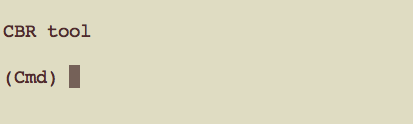
\includegraphics[width=0.6\linewidth]{images/main}
    \caption{CBR Interface}
    \label{fig:main}
\end{figure}

If we type \emph{help} AICS will prompt the different functions (see Figure \ref{fig:cbrfunctions}.

\begin{figure}[htb]
    \center
    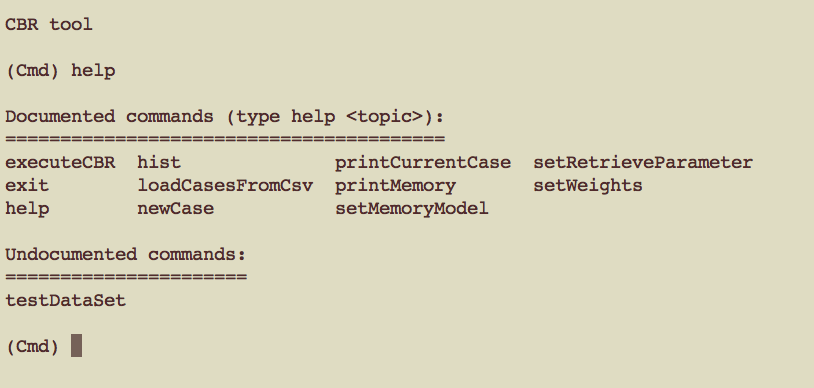
\includegraphics[width=1\linewidth]{images/cbrfunctions}
    \caption{CBR Functions}
    \label{fig:cbrfunctions}
\end{figure}

Hence we will outline the functionality of each functions. These functionalities are listed with its description here:

\begin{itemize}
    \item \begin{description}
            \item[loadCasesFromCsv] Allows to load a dataset
        \end{description}
    \item \begin{description}
        \item[newCase] Allows to introduce a new case to be tested
    \end{description}              
    \item \begin{description}
        \item[setWeights] Allows to assign a weight to each attribute
    \end{description}              
    \item \begin{description}
        \item[setMemoryModel] Allows to select between use a flatMemory or a kdTree
    \end{description}              
    \item \begin{description}
        \item[setRetrieveParameter] Allows to set the number of cases to retrieve in the retrieval phase
    \end{description}              
    \item \begin{description}
        \item[executeCBR] Executes the CBR over the new case introduced    
    \end{description}              
    \item \begin{description}
        \item[testDataSet] Makes different tests over the dataset introduced by splitting it into train and test data sets with different ratios    
    \end{description}              
    \item \begin{description}
        \item[printCurrentCase] Print the current case loaded
    \end{description}              
    \item \begin{description}
        \item[printMemory] Print the cases loaded at the library of cases 
    \end{description}              
    \item \begin{description}
        \item[hist] Shows the last commands used
    \end{description}              
    \item \begin{description}
        \item[help] Giving a function as a parameter it provides information about that function
    \end{description}             
    \item \begin{description}
        \item[exit] Close the CBR tool
    \end{description}              
\end{itemize}

At this point we will outlinen in the following section a guided example in order to better understand how it works.
\section{A guided example}


Let's go through the basic functionality of our CBR system. In order to do so we will use the Iris data set as guided example.

To start AICS the user needs to execute the CBR.py script using a python interpreter:
\begin{verbatim}
    >> ipython ./CBR.py
\end{verbatim}
This executes an interactive shell where the user can interact with the system:
\begin{verbatim}
    CBR tool

    (Cmd)
\end{verbatim}
Typing \texttt{help} we get a list of the available commands
\begin{verbatim}
    (Cmd) help
    
    Documented commands (type help <topic>)
    ========================================
    executeCBR  hist              printCurrentCase  setRetrieveParameter
    exit        loadCasesFromCsv  printMemory       setWeights
    help        newCase           setMemoryModel

\end{verbatim}

For more information about a command just type: $\texttt{help <commandName>}$. Let's begin loading the Iris data set from a CSV file into the system. To load a set of cases from a CSV file use the \texttt{loadCasesFromCsv} command:
\begin{verbatim}
    (Cmd) loadCasesFromCsv datasets/iris.data.csv
\end{verbatim}

The command takes the file path as a string and starts an interactive process so the user can set the variable types and names. The following message will pop up in the screen:
\begin{verbatim}
    We need to know the kind of attributes present in the CSV 
    file. Introduce such types of variables. Example:
        r,r,r,c
    In this case the csv file will have 4 columns, being the 
    three first real values and the last one a categorical one.

    Introduce the kind of variables:
\end{verbatim}

In this case we have 5 columns with 4 real valued attributes and the categorical labels:
\begin{verbatim}
    Introduce the kind of variables: r,r,r,r,c
\end{verbatim}

The next step is to introduce the name of all the attributes including the label
\begin{verbatim}
    Introduce the names of the variables: sepal-length, 
                                          sepal-width, 
                                          petal-length, 
                                          petal-width, 
                                          specie
\end{verbatim}

Finally, we need to introduce the position of the label within the attributes, in this case it is the 5th attribute:
\begin{verbatim}
    Now we need to know which parameter specifies the solution of 
    the case. Indicate that through a number
    Introduce the variable that is the solution (number): 5
\end{verbatim}

This last step finishes the load of a CSV. 

The next step the user may want to take is to set the weights for the attributes, this step is optional and if the user does not specify any custom weights all the attributes will be given equal weight. Let's add some random weights using the \texttt{setWeights} command to illustrate the process:
\begin{verbatim}
    (Cmd) setWeights
    Introduce petal-width:
    3.14
    Introduce sepal-width:
    2.71
    Introduce sepal-length:
    1.414
    Introduce petal-length:
    1.618
\end{verbatim}

Before introducing new cases and running the CBR loop the user can set some more settings to customize the CBR process. For instance, the user can set the number of similar cases that will be fetched in the retrieve step:
\begin{verbatim}
    (Cmd) setRetrieveParameter 5
\end{verbatim}
We have set the retrieve parameter to 5, this step is also optional and the default value is 1.

In addition the user can also select the library structure that is used to store and retrieve the case: flat memory or hierarchical memory. To change from one to another use the \texttt{setMemoryModel (flat | hierarchical)} command.
\\

Once the CBR system has been set the user can start introducing new cases. We can input them using the $\texttt{newCase}$ command:
\begin{verbatim}
    (Cmd) newCase
    Introduce petal-width:
    3.0
    Introduce sepal-width:
    3.5
    Introduce sepal-length:
    4.0
    Introduce petal-length:
    4.1
\end{verbatim}

Now that we have loaded a new case we can call the \texttt{executeCBR}:
\begin{verbatim}
   ====== CASE ======
   -- Attributes
   petal-width :  1.5
   sepal-width :  3.0
   sepal-length :  5.4
   petal-length :  4.5
   -- Label
   specie :  Iris-versicolor
   ==================
   sim:  0.312895672112

   ====== CASE ======
   -- Attributes
   petal-width :  1.7
   sepal-width :  2.5
   sepal-length :  4.9
   petal-length :  4.5
   -- Label
   specie :  Iris-virginica
   ==================
   sim:  0.31409347541
   
   ====== CASE ======
   -- Attributes
   petal-width :  1.6
   sepal-width :  3.4
   sepal-length :  6.0
   petal-length :  4.5
   -- Label
   specie :  Iris-versicolor
   ==================
   sim:  0.314331159615
   
   ====== CASE ======
   -- Attributes
   petal-width :  2.3
   sepal-width :  3.4
   sepal-length :  6.2
   petal-length :  5.4
   -- Label
   specie :  Iris-virginica
   ==================
   sim:  0.31532658149
   
   ====== CASE ======
   -- Attributes
   petal-width :  2.4
   sepal-width :  3.4
   sepal-length :  6.3
   petal-length :  5.6
   -- Label
   specie :  Iris-virginica
   ==================
   sim:  0.324688551
   
   ADAPTATION - Result (Solution):
   Iris-virginica
\end{verbatim}

The solution of the new case is then \texttt{Iris-virginica}.
\\

After the system has presented what it considers the best solution, the user is asked to input the correct solution value for the new case, so that the system will know if it has given the right or wrong answer.
\begin{verbatim}
-- Label
specie :  Iris-versicolor
Utility:  0
Evaluation:  True
==================
sim:  0.433615819209
ADAPTATION - Result (Solution):
Iris-versicolor
Introduce the real solution:Iris-setosa
\end{verbatim}


After this step, the system takes control of the remaining evaluation/retain phase of the CBR, and loops back to the beginning state, ready to admit new cases, while its memory is now, ideally, more capable of providing a correct answer to a new case, and even more with each iteration of the CBR process.

Furthermore, there is one functionality that tests the CBR with the dataset loaded to check its accuracy by executing several tests. After the execution of such tests it outlines the results giving to the user the accuracy reached for each one. Thus, the user could know which are the best settings of the method for the given dataset.


\end{document}


